\documentclass[11pt]{article}
\usepackage[T1]{fontenc}
\usepackage{lmodern}
\usepackage{amsmath,amssymb,amsthm,mathtools}
\usepackage[letterpaper,margin=1in]{geometry}
\usepackage{microtype}
\usepackage{enumitem}
\usepackage{booktabs}
\usepackage{graphicx}
\usepackage{tikz}
\usetikzlibrary{arrows.meta,calc,positioning}
\usepackage{xcolor}
\definecolor{linkblue}{HTML}{23527C}
\definecolor{parentblue}{HTML}{28698D}
\definecolor{childorange}{HTML}{B76223}
\usepackage[colorlinks=true,linkcolor=linkblue,citecolor=linkblue,urlcolor=linkblue]{hyperref}
\usepackage[capitalise,noabbrev]{cleveref}
\hypersetup{pdftitle={Thompson's group F is nonamenable},pdfauthor={OpenAI}}

\newcommand{\R}{\mathbb R}
\newcommand{\N}{\mathbb N}
\newcommand{\Z}{\mathbb Z}
\newcommand{\norm}[1]{\lVert #1\rVert}
\newcommand{\ip}[2]{\langle #1,#2\rangle}
\newcommand{\id}{\mathrm{id}}
\DeclareMathOperator{\Lip}{Lip}
\DeclareMathOperator{\dist}{dist}
\newtheorem{theorem}{Theorem}[section]
\newtheorem{lemma}[theorem]{Lemma}
\newtheorem{proposition}[theorem]{Proposition}
\newtheorem{corollary}[theorem]{Corollary}
\theoremstyle{definition}
\newtheorem{definition}[theorem]{Definition}
\newtheorem{remark}[theorem]{Remark}
\numberwithin{equation}{section}
\setlist[itemize]{topsep=4pt,itemsep=2pt,parsep=0pt}
\setlist[enumerate]{topsep=4pt,itemsep=2pt,parsep=0pt}
\setlength{\emergencystretch}{2em}


\title{Thompson's group \(F\) is nonamenable}
\author{OpenAI}
\date{September 23, 2026}

\begin{document}
\maketitle
\begin{abstract}
We prove that Thompson's group \(F\) is nonamenable. This confirms
Geoghegan's conjecture and resolves the amenability problem for \(F\).
\end{abstract}

\section{Introduction}
\label{sec:introduction}

Thompson's group \(F\) consists of the increasing piecewise linear
homeomorphisms of \([0,1]\) with finitely many pieces, dyadic rational
breakpoints, and slopes in \(2^{\Z}\). We use the multiplication convention
\(hg=h\circ g\) and regard \(F\) as a discrete group.

A discrete group \(G\) is \emph{amenable} if its bounded real-valued
functions admit a positive normalized left-invariant mean: a linear
functional \(M:\ell^\infty(G;\R)\to\R\) satisfying \(M(1)=1\),
\(M(\varphi)\ge0\) whenever \(\varphi\ge0\), and
\(M(g\mapsto\varphi(hg))=M(\varphi)\) for every \(h\in G\).
This invariant-mean viewpoint belongs to the classical theory developed
by von Neumann and Day \cite{vonNeumann1929,Day1957}.
We use the following forward implication of the F\o lner criterion
\cite{Folner1955}: if \(G\) is amenable, then for every finite
\(S\subset G\) and every \(\varepsilon>0\), there is a nonempty finite
\(A\subset G\) such that
\begin{equation}\label{eq:folner}
  \frac{|hA\mathbin{\triangle}A|}{|A|}<\varepsilon
  \qquad(h\in S).
\end{equation}
The modern left-translation formulation in
\cite[Theorem~1.2]{Moore2013} bounds the sum of these ratios and hence
implies each strict individual bound by taking a smaller tolerance.
Thus amenability requires finite sets
whose relative boundaries are simultaneously small under any fixed
finite family of translations.

Thompson introduced \(F\) in 1965; an early published construction appears
in McKenzie and Thompson \cite{McKenzieThompson1973}, with the identification
explained by Cannon, Floyd, and Parry \cite[pp.~215--216]{CannonFloydParry1996}.
The latter authors record Geoghegan's 1979 conjecture that \(F\) is
nonamenable \cite[p.~227]{CannonFloydParry1996}. We prove this conjecture.

\begin{theorem}\label{thm:main}
Thompson's group \(F\) is not amenable.
\end{theorem}

\paragraph{Context and prior work.}
Two classical structural facts help explain the difficulty of the
amenability problem. Brin and Squier show that \(F\) contains no
nonabelian free subgroup \cite[Theorem~3.1]{BrinSquier1985}, so the familiar
free-subgroup obstruction does not apply. Yet \(F\) is not elementary
amenable \cite[Theorem~4.10]{CannonFloydParry1996}: it lies outside the class
generated by finite and abelian groups under subgroups, quotients,
extensions, and directed unions. Neither fact decides ordinary
amenability. The group also has strong topological finiteness properties:
Brown and Geoghegan construct a classifying space with finitely many
cells in each dimension \cite{BrownGeoghegan1984}.

Finite approximations have provided several ways to study the remaining
question. Moore proves tower lower bounds on the sizes of possible
F\o lner sets \cite[Theorem~1.1]{MooreFolner2013} and characterizes
amenability of \(F\) by a scalar convex Ramsey property for finite rooted
ordered binary trees \cite[Theorem~3.1]{Moore2013}. Guba improves densities
of finite Cayley subgraphs \cite{Guba2025Density} and derives restrictions
on right-invariant means from a partition into seven diagram-defined
classes \cite{Guba2026}. From an operator-algebraic
direction, Haagerup and Olesen prove that simplicity of the reduced group
\(C^*\)-algebra of Thompson's group \(T\) would imply nonamenability of
\(F\) \cite[Theorem~5.5]{HaagerupOlesen2017}. These results expose constraints
on amenability through finite sets, trees, diagrams, and representations.
The proof below uses finite dyadic partitions and scalar correlations of
Hilbert-valued colors.

There have also been claims of a complete resolution in both directions.
Akhmedov's 2021 version claims nonamenability through a height-function
criterion \cite{Akhmedov2021}. Shavgulidze claimed amenability
\cite{Shavgulidze2009}; Moore identified errors in that approach
\cite{Moore2011Critique}. Moore separately withdrew an amenability claim
after Akhmedov identified an error in Lemma~4.13 of that manuscript
\cite{Moore2012Withdrawn}. That withdrawal concerns a different work from
his published Ramsey characterization cited above.

\paragraph{Proof strategy.}
The proof turns approximate translation invariance of finite averages of
scalar functions on \(F\) into an approximate fixed point of a Lipschitz
map on a Hilbert ball. The
following infinite-dimensional phenomenon supplies a map for which that
conclusion is impossible.

\begin{lemma}[Benyamini--Sternfeld]\label{lem:displacement}
There are a real Hilbert space \(H\), a Lipschitz map \(f:B\to B\) on its
closed unit ball, and a constant \(\delta>0\) such that
\[
  \norm{f(x)-x}\ge\delta\qquad(x\in B).
\]
\end{lemma}

Benyamini and Sternfeld prove this assertion for every infinite-dimensional
normed space \cite[Theorem, part~(3), p.~439]{BenyaminiSternfeld1983}.
For completeness, Appendix~\ref{app:auxiliary} constructs such a map on
\(L^2([0,1];\R^2)\) with \(\delta=1/2\), including all the needed
Lipschitz estimates.

Fix this map \(f\), a positive Lipschitz constant \(L\), and a large
integer \(D\). A basic dyadic interval is a cell of a uniform dyadic
partition, and a basic partition is a finite partition into such cells.
Choose \(D\) basic intervals with positive gaps between them and endpoints
in \((0,1)\), called parents. Put an affine copy of this family inside
each parent, calling the copies descendants. When a parent is a union
of partition cells, restricting to it and stretching back to \([0,1]\)
gives its normalized restriction. Color each basic partition recursively
by applying \(f\) to the mean of its parent-restriction colors when all
these restrictions are defined, and by zero otherwise. Proper
restriction decreases the number of cells, so the recursion is well
founded. For a sufficiently fine image partition under \(g\in F\), its
parent colors \(X_i\) and descendant colors \(Y_{ij}\) therefore satisfy
\[
 m=\frac1D\sum_{i=1}^D X_i,\qquad
 z_i=\frac1D\sum_{j=1}^D Y_{ij},\qquad
 X_i=f(z_i)\quad(1\le i\le D).
\]

The group \(F\) can carry any ordered pair of separated basic intervals
with endpoints in \((0,1)\) affinely onto any other such pair. Choose a
finite set \(S\) of these transports comparing every separated pair among
the parents and descendants with one reference pair. The set \(S\) is
fixed before the arbitrary nonempty
finite set \(A\subset F\); only the common partition level, chosen fine
enough for \(A\cup SA\), may depend on \(A\). Write \(\eta\) for the
largest relative \(S\)-boundary of \(A\). Exact covariance of normalized
restrictions and finite-average cancellation make all averaged scalar
correlations of separated interval colors differ from one common value
by at most \(\eta\).

Expand the average over \(A\) of \(\norm{z_i-m}^2\). The common
correlation cancels; diagonal and nested pairs occupy only a fraction
\(1/D\) of each relevant sum, as Figure~\ref{fig:mixed-pairs} illustrates.
Unit-ball bounds control those exceptions, giving a universal constant
times \(D^{-1}+\eta\). Since \(m\) is also the mean of the \(f(z_i)\),
convexity and Lipschitz continuity bound the average squared displacement
\(\norm{m-f(m)}^2\) by a constant times \(L^2(D^{-1}+\eta)\).
For large \(D\) and small \(\eta\), this contradicts the uniform lower
bound \(\delta^2\). Section~\ref{sec:proof} makes the argument precise and proves a
uniform positive boundary bound in Proposition~\ref{avg:boundary},
contradicting \eqref{eq:folner}.

Section~\ref{sec:consequences} records consequences for uniformly bounded
representations and percolation, using separate companion theorems.

\section{Recursive colors and finite averages}\label{sec:proof}

We prove Theorem~\ref{thm:main} using the map supplied by
Lemma~\ref{lem:displacement}.  The argument uses a single finite average
over the group.  We first record the dyadic facts that make its
correlations comparable.

\subsection{Dyadic partitions and affine transport}\label{sec:dyadic}

We use the standard dyadic-partition model of $F$; see
\cite[Section~2, Lemma~2.2]{CannonFloydParry1996}. We record the
restriction and pair-transport facts needed for the finite averages.

A \emph{basic dyadic interval} is an interval
\[
  [k2^{-r},(k+1)2^{-r}]\subseteq[0,1],
  \qquad r\in\N\cup\{0\},\quad 0\leq k<2^r.
\]
A \emph{basic partition} is a finite partition of $[0,1]$ into such
intervals; cells may share endpoints.  Its mesh is the greatest length
of a cell.  A partition $T$ \emph{respects} an interval $I$ if $I$ is a
union of cells of $T$.

For a basic interval $I$, let $s_I:[0,1]\to I$ be the increasing affine
map, and write $I\cdot J=s_I(J)$.  If $T$ respects $I$, define its
normalized restriction by
\[
  T_I=\{s_I^{-1}(K):K\in T,\ K\subseteq I\}.
\]
Both $I\cdot J$ and the cells of $T_I$ are basic dyadic intervals.
Indeed, if $I$ has length $2^{-r}$, a basic cell contained in $I$ has
length $2^{-s}$ with $s\geq r$; applying $s_I^{-1}$ gives a cell of
length $2^{-(s-r)}$ whose left endpoint is a multiple of that length.
The affine charts satisfy $s_{I\cdot J}=s_I\circ s_J$.  Consequently,
whenever $T$ respects both $I$ and $I\cdot J$, the partition $T_I$
respects $J$ and
\begin{equation}\label{dyad:restriction}
  (T_I)_J=T_{I\cdot J}.
\end{equation}

Let $T^{(n)}$ be the uniform partition of $[0,1]$ into intervals of
length $2^{-n}$.  For $g\in F$, the notation $gT^{(n)}$ denotes the
partition formed by the images of these cells.

\begin{lemma}\label{dyad:eventual}
For each $g\in F$, the partitions $gT^{(n)}$ are basic for all
sufficiently large $n$, and their meshes tend to zero.  In particular,
given a finite set $K\subset F$ and a finite family $\mathcal J$ of
basic intervals, there is an $n_0$ such that $gT^{(n)}$ is basic and
respects every member of $\mathcal J$ whenever $g\in K$ and $n\geq n_0$.
\end{lemma}

\begin{proof}
The image under $g$ of each breakpoint is dyadic: starting from
$g(0)=0$, sum the increments on the preceding linear pieces, each a
power of two times a dyadic length.  Thus every linear piece has the
form $x\mapsto 2^q x+b$ with $q\in\mathbb Z$ and $b$ dyadic.  Choose
$n$ large enough to resolve all breakpoints, to have $n\geq q$ on
every piece, and to make each corresponding $b$ an integer multiple
of $2^{q-n}$.  The image of each uniform cell is then a basic interval
of length $2^{q-n}$.  There are finitely many slopes, so the mesh tends
to zero.

Two basic intervals with intersecting interiors are nested.  Hence
a basic partition of mesh smaller than the length of a basic
interval $I$ respects $I$: every cell whose interior meets that of
$I$ must be contained in $I$.  Apply this observation to the
finitely many intervals in $\mathcal J$, and then take the maximum
of the finitely many thresholds for $g\in K$.
\end{proof}

Write $I<J$ when $\max I<\min J$; in particular this notation requires
a positive gap.  An interval is \emph{internal} if both its endpoints
lie in $(0,1)$.

\begin{lemma}\label{dyad:transport}
If $I<J$ and $I'<J'$ are pairs of internal basic intervals, there is
an $h\in F$ whose restrictions carry $I$ affinely onto $I'$ and $J$
affinely onto $J'$.
\end{lemma}

\begin{proof}
The two selected intervals leave three complementary gaps, all of
positive length and with dyadic endpoints.  Partition each gap into
basic cells, for example by a sufficiently fine uniform dyadic
grid.  Do this for both pairs.  Within each corresponding pair of
gaps, equalize the numbers of cells by successively bisecting cells
on the side with fewer cells.  Each bisection increases the number
by one.  The source and target partitions now have the same number
of cells, with the two selected intervals in matching positions.
Map corresponding cells increasingly and affinely.  All
breakpoints are dyadic and all slopes are ratios of basic lengths,
hence powers of two.  This defines the required element of $F$.
\end{proof}

The relevant covariance is exact.  If $h$ carries $I$ affinely onto
$I'$, then $h\circ s_I=s_{I'}$.  Thus, if $gT^{(n)}$ and
$(hg)T^{(n)}$ are basic and respect $I$ and $I'$, respectively,
\begin{equation}\label{dyad:covariance}
  \bigl((hg)T^{(n)}\bigr)_{I'}=(gT^{(n)})_I.
\end{equation}
Here, as throughout, $hg=h\circ g$.  To verify the equality, match
each source cell $C$ with its image $h(C)$ and apply
$s_{I'}^{-1}\circ h=s_I^{-1}$ on $I$.

\subsection{The recursive coloring}\label{sec:coloring}

Fix a real Hilbert space $H$, its closed unit ball $B$, and a
Lipschitz map $f:B\to B$ as in Lemma~\ref{lem:displacement}.  Fix
$L>0$ and $\delta>0$ such that
\begin{equation}\label{color:map}
  \norm{f(x)-f(y)}\leq L\norm{x-y},\qquad
  \norm{f(x)-x}\geq\delta
  \quad(x,y\in B).
\end{equation}
Choose an integer $D\geq2$ so that
\begin{equation}\label{color:parameters}
  D>\frac{4L^2}{\delta^2}.
\end{equation}
Choose internal basic intervals $I_1<\cdots<I_D$.  Such a family
exists for every finite $D$: take $2^r>2D$ and use
$I_j=[(2j-1)2^{-r},2j2^{-r}]$.

Define a color $p(T)\in B$ for every basic partition $T$ by induction
on its number of cells:
\begin{equation}\label{color:recursion}
  p(T)=
  \begin{cases}
  \displaystyle f\left(\frac1D\sum_{j=1}^D p(T_{I_j})\right),
       &\text{if $T$ respects every $I_j$},\\[6pt]
  0,   &\text{otherwise}.
  \end{cases}
\end{equation}
This induction is well founded.  In the first case each $T_{I_j}$
has strictly fewer cells than $T$, since $I_j$ is internal and $T$
has cells outside it.  The average of the previously defined
colors belongs to the convex ball $B$, so the argument of $f$ is
always in its domain, and $p(T)\in B$.

For the displayed choice $|I_j|=2^{-r}$, the one-cell partition
$T^{(0)}$ has color zero, while
\[
  p(T^{(r)})=f(0),\qquad
  p(T^{(2r)})=f(f(0)).
\]
Indeed, normalizing a restriction to any $I_j$ changes these uniform
partition levels from $r$ to $0$ and from $2r$ to $r$, respectively.

We use the finite family of parent intervals and their descendants
\[
  \mathcal I=\{I_i:1\leq i\leq D\}
       \cup\{I_i\cdot I_j:1\leq i,j\leq D\}.
\]
All these intervals are internal.  Call $(n,g)$ \emph{admissible}
if $gT^{(n)}$ is a basic partition respecting every member of
$\mathcal I$.  For every $n$, every $g\in F$, and every
$I\in\mathcal I$, define
\begin{equation}\label{color:global}
  X_I^{(n)}(g)=
  \begin{cases}
    p\bigl((gT^{(n)})_I\bigr),&\text{if $(n,g)$ is admissible},\\
    0,&\text{otherwise}.
  \end{cases}
\end{equation}
In particular these are globally defined $B$-valued functions.
Their scalar correlations
\[
  \varphi_{I,J}^{(n)}(g)
     =\ip{X_I^{(n)}(g)}{X_J^{(n)}(g)}
\]
are defined on all of $F$ and have absolute value at most one.
By Lemma~\ref{dyad:eventual}, every finite set of group elements is
admissible at one common sufficiently large level $n$.

\subsection{A uniform boundary bound}\label{sec:boundary}

For every
ordered pair $I<J$ in $\mathcal I$, choose, using
Lemma~\ref{dyad:transport}, an element $h_{I,J}\in F$ carrying
$I,J$ affinely onto $I_1,I_2$, respectively.  Let $S$ be the finite
set of these elements.  All choices so far, in particular $S$, are
independent of the finite set to be tested.

For any nonempty finite \(A\subset F\), any \(h\in F\), and any
\(\varphi:F\to[-1,1]\), cancellation over \(hA\cap A\) gives
\begin{equation}\label{eq:finite-translation}
 \left|\frac1{|A|}\sum_{g\in A}\varphi(hg)
       -\frac1{|A|}\sum_{g\in A}\varphi(g)\right|
 \le\frac{|hA\mathbin{\triangle}A|}{|A|}.
\end{equation}
This is the finite-average comparison we will apply to the scalar
correlations.

\begin{proposition}\label{avg:boundary}
For every nonempty finite set $A\subset F$,
\begin{equation}\label{avg:boundary-bound}
  \max_{h\in S}\frac{|hA\mathbin{\triangle}A|}{|A|}
  \geq \frac{\delta^2/L^2-4/D}{4(1-1/D)}>0.
\end{equation}
\end{proposition}

\begin{proof}
Fix such a set $A$ and put
\begin{equation}\label{avg:defect}
  \eta=\max_{h\in S}\frac{|hA\mathbin{\triangle}A|}{|A|}.
\end{equation}
Choose a single $n$ for which $(n,g)$ is admissible for all
\[
  g\in A\cup SA,
  \qquad SA=\bigcup_{h\in S}hA.
\]
This choice is possible because that union is finite; the level $n$
may depend on $A$.  We now fix this $n$, omit its superscript, and write
\[
  \mathbb E_A\psi=\frac1{|A|}\sum_{g\in A}\psi(g),
  \qquad
  \alpha=\mathbb E_A\varphi_{I_1,I_2}.
\]
\paragraph{Comparing correlations.}
For $I<J$ in $\mathcal I$ and $g\in A$, admissibility of both $g$
and $h_{I,J}g$, together with \eqref{dyad:covariance}, gives
\[
  X_I(g)=X_{I_1}(h_{I,J}g),\qquad
  X_J(g)=X_{I_2}(h_{I,J}g).
\]
It follows that $\varphi_{I,J}(g)
=\varphi_{I_1,I_2}(h_{I,J}g)$.  Apply
\eqref{eq:finite-translation} to the globally bounded function
$\varphi_{I_1,I_2}$ and use \eqref{avg:defect}.  We obtain
\begin{equation}\label{avg:correlation}
  \left|\mathbb E_A\ip{X_I}{X_J}-\alpha\right|
       \leq\eta
  \qquad\text{whenever $I,J\in\mathcal I$ are strictly separated}.
\end{equation}
The reversed order follows from symmetry of the real inner
product.  No condition is imposed on nested pairs.  Also, a
transport $h_{I,J}$ need not preserve the other intervals in
$\mathcal I$: admissibility was required separately at its source
and target group elements.

\paragraph{The variance estimate.}

For $g\in A$, put
\[
  m(g)=\frac1D\sum_{k=1}^D X_{I_k}(g),\qquad
  z_i(g)=\frac1D\sum_{j=1}^D X_{I_i\cdot I_j}(g)
       \quad(1\leq i\leq D).
\]
These vectors lie in $B$.  Admissibility ensures that the partition
$(gT^{(n)})_{I_i}$ respects each $I_j$.  Applying the recursion and
\eqref{dyad:restriction} therefore yields the exact identities
\begin{equation}\label{avg:recursive-identity}
  X_{I_i}(g)=f(z_i(g))\qquad(g\in A, 1\leq i\leq D).
\end{equation}
Consequently, for every $g\in A$, the displacement bound, the
convexity of the squared norm, and the Lipschitz bound give
\begin{align}
  \delta^2
  &\leq\norm{m(g)-f(m(g))}^2\notag\\
  &=\left\|\frac1D\sum_{i=1}^D
                   \bigl(f(z_i(g))-f(m(g))\bigr)\right\|^2\notag\\
  &\leq\frac1D\sum_{i=1}^D
                   \norm{f(z_i(g))-f(m(g))}^2\notag\\
  &\leq\frac{L^2}{D}\sum_{i=1}^D\norm{z_i(g)-m(g)}^2.
       \label{avg:displacement}
\end{align}

We bound the finite average of each squared distance in the last
line.  In the expansion of $\norm{m}^2$, the $D(D-1)$
off-diagonal terms pair strictly separated parents, so
\eqref{avg:correlation} applies.  Each of the $D$ diagonal terms
is at most one.  The same statements hold for the siblings in
$\norm{z_i}^2$.  Hence
\begin{align}
  \mathbb E_A\norm{m}^2
       &\leq\left(1-\frac1D\right)(\alpha+\eta)+\frac1D,
       \label{avg:parent-bound}\\
  \mathbb E_A\norm{z_i}^2
       &\leq\left(1-\frac1D\right)(\alpha+\eta)+\frac1D.
       \label{avg:child-bound}
\end{align}
In the mixed term
\[
  \ip{z_i}{m}
    =\frac1{D^2}\sum_{j=1}^D\sum_{k=1}^D
                  \ip{X_{I_i\cdot I_j}}{X_{I_k}},
\]
the $D(D-1)$ terms with $k\ne i$ pair strictly separated
intervals.  Each has average at least $\alpha-\eta$.
The remaining $D$ terms pair a descendant with its own parent;
each is at least $-1$ by the unit-ball bound.  Figure~\ref{fig:mixed-pairs}
shows this division of the mixed pairs.  Thus
\begin{equation}\label{avg:mixed-bound}
  \mathbb E_A\ip{z_i}{m}
    \geq\left(1-\frac1D\right)(\alpha-\eta)-\frac1D.
\end{equation}
\begin{figure}[tbp]
\centering
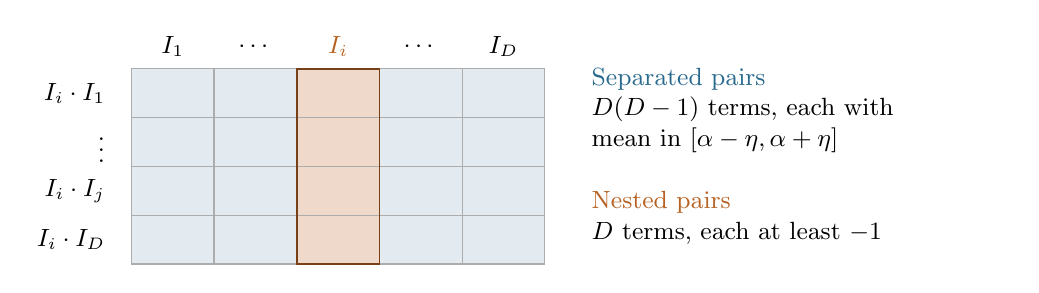
\begin{tikzpicture}[x=1.05cm,y=0.62cm,font=\small]
  \foreach \x in {0,1,2,3,4} {
    \foreach \y in {0,1,2,3} {
      \fill[parentblue!13] (\x,\y) rectangle +(1,1);
    }
  }
  \fill[childorange!24] (2,0) rectangle (3,4);
  \draw[gray!65,thin] (0,0) grid[xstep=1,ystep=1] (5,4);
  \draw[childorange!65!black,semithick] (2,0) rectangle (3,4);
  \node at (0.5,4.45) {$I_1$};
  \node at (1.5,4.45) {$\cdots$};
  \node[childorange] at (2.5,4.45) {$I_i$};
  \node at (3.5,4.45) {$\cdots$};
  \node at (4.5,4.45) {$I_D$};
  \node[anchor=east] at (-0.2,3.5) {$I_i\cdot I_1$};
  \node[anchor=east] at (-0.2,2.5) {$\vdots$};
  \node[anchor=east] at (-0.2,1.5) {$I_i\cdot I_j$};
  \node[anchor=east] at (-0.2,0.5) {$I_i\cdot I_D$};
  \node[anchor=west,align=left,text width=5.2cm] at (5.45,3.15)
    {\textcolor{parentblue}{Separated pairs}\\
     \(D(D-1)\) terms, each with\\
     mean in \([\alpha-\eta,\alpha+\eta]\)};
  \node[anchor=west,align=left,text width=5.2cm] at (5.45,0.95)
    {\textcolor{childorange}{Nested pairs}\\
     \(D\) terms, each at least \(-1\)};
\end{tikzpicture}
\caption{For fixed \(i\), the \((j,k)\) entry is
\(\ip{X_{I_i\cdot I_j}}{X_{I_k}}\). Rows index the children of
\(I_i\) and columns index all parents; the grid is schematic.
Only column \(i\) contains nested pairs, a fraction \(1/D\) of the
\(D^2\) terms.}
\label{fig:mixed-pairs}
\end{figure}

Expanding the squared distance and using
\eqref{avg:parent-bound}--\eqref{avg:mixed-bound}, the coefficients
of $\alpha$ cancel and give
\begin{equation}\label{avg:variance}
  \mathbb E_A\norm{z_i-m}^2
    \leq\frac4D+4\left(1-\frac1D\right)\eta
    \qquad(1\leq i\leq D).
\end{equation}
This estimate does not require any sign assumption on $\alpha$.

Average \eqref{avg:displacement} over $A$ and apply
\eqref{avg:variance}:
\begin{align*}
  \delta^2
  &\leq\frac{L^2}{D}\sum_{i=1}^D
                 \mathbb E_A\norm{z_i-m}^2\\
  &\leq L^2\left(\frac4D+4\left(1-\frac1D\right)\eta\right).
\end{align*}
Rearranging proves \eqref{avg:boundary-bound}; its right-hand side is
positive by \eqref{color:parameters} and does not depend on $A$.
\end{proof}

\begin{proof}[Proof of Theorem~\ref{thm:main}]
The fixed finite set $S$ and the uniform positive lower bound in
Proposition~\ref{avg:boundary} violate the F\o lner criterion
\eqref{eq:folner}.  Hence $F$ is not amenable.
\end{proof}

\section{Consequences}\label{sec:consequences}

Theorem~\ref{thm:main} allows us to apply two companion results for
nonamenable groups. The first concerns representations that are uniformly
close to being isometric but cannot be made unitary by an equivalent
Hilbert norm. The second concerns percolation on the simple Cayley graphs of \(F\)
associated with finite symmetric generating sets.
Neither companion result is used in the proof of nonamenability.

\subsection{Uniformly bounded representations}

\begin{corollary}\label{cor:nonunitarizable}
For every \(\varepsilon>0\), there are a separable complex Hilbert space
\(H\) and a representation \(\pi:F\to\mathrm{GL}(H)\) such that
\(\sup_{g\in F}\norm{\pi(g)}\le1+\varepsilon\), but no bounded invertible
operator \(S\) on \(H\) makes every \(S\pi(g)S^{-1}\) unitary.
\end{corollary}

\begin{proof}
The group \(F\) is countable, by its finite dyadic piecewise linear
description, and nonamenable by Theorem~\ref{thm:main}, so the conclusion
follows from the companion unitarizability theorem
\cite[Theorem~1.1]{OpenAIUnitarizability2026}.
\end{proof}

\subsection{Percolation on Cayley graphs}

For a finite symmetric generating set \(S\subset F\setminus\{\id\}\), let
\(G_S\) be the simple undirected Cayley graph with edges \(\{x,xs\}\).
In Bernoulli bond percolation on this fixed graph, each edge is independently
open with probability \(p\). Write \(p_c\) for the threshold for existence
of an infinite open cluster and \(p_u\) for the threshold for almost-sure
uniqueness of the infinite open cluster. The connection kernel
\(T_p(x,y)=\mathbb P_p(x\leftrightarrow y)\) acts on counting-measure
\(\ell^2(F)\), initially on finitely supported functions by summation over
\(y\); put \(p_{2\to2}=\sup\{p\in[0,1]:T_p\text{ is bounded on }\ell^2(F)\}\).

\begin{corollary}\label{cor:percolation}
For every such generating set \(S\),
\[
  \norm{T_{p_c}}_{2\to2}<\infty,\qquad p_c<p_{2\to2}\le p_u.
\]
For each fixed \(p\in(p_c,p_u)\), there are almost surely infinitely many
infinite open clusters. Moreover, there are deterministic
\(p_c<p_1<p_2<1\), depending on \(S\), such that in the coupling with
independent uniform \([0,1]\) edge labels \(U_e\), opening \(e\) when \(U_e\le p\),
there are almost surely infinitely many infinite open clusters
simultaneously for every \(p\in[p_1,p_2]\).
\end{corollary}

\begin{proof}
Apply the companion percolation result
\cite[Corollary~1.2]{OpenAIPercolation2026} to \(F\), which is nonamenable
by Theorem~\ref{thm:main}.
\end{proof}


\appendix
\section{An explicit map with positive displacement}\label{app:auxiliary}

We give a direct construction of the map needed in
Lemma~\ref{lem:displacement}. This proves the Hilbert-space instance of
the Benyamini--Sternfeld theorem~\cite{BenyaminiSternfeld1983} directly.
The aim is to construct a Lipschitz map
$G:B\to H$ bounded away from zero and equal to the identity when
$\norm{x}\ge1/2$. Then $f(x)=-G(x)/\norm{G(x)}$ has the required
displacement. A tube about a curve with a bounded tail supplies $G$.

\begin{proposition}\label{aux:map}
Let $H=L^2([0,1];\R^2)$ be a real Hilbert space and let
$B=\{x\in H:\norm{x}\le1\}$. There is a globally Lipschitz map $f:B\to B$
such that
\[
  \norm{f(x)}=1,
  \qquad \norm{f(x)-x}\ge\frac12
  \quad(x\in B).
\]
\end{proposition}

Define functions on $\R$ by
\[
 a(t)=
 \begin{cases}
 t/8,&t\le2,\\
 5/16-(3-t)^2/16,&2<t<3,\\
 5/16,&t\ge3,
 \end{cases}
 \qquad
 \theta(t)=
 \begin{cases}
 0,&t\le1,\\
 (t-1)^2/2,&1<t<2,\\
 t-3/2,&t\ge2.
 \end{cases}
\]
For $w\in[0,1]$, put
\[
 v(t)(w)=(\cos(\theta(t)w),\sin(\theta(t)w)),
 \qquad \gamma(t)=a(t)v(t).
\]
Thus $\norm{v(t)}=1$, $\gamma(0)=0$, and $\gamma$ follows a straight line
for $t\le1$; its tail for $t\ge1$ lies in the ball of radius $5/16$.
The next lemma shows that, although the positive tail is bounded, curve
points whose parameters differ by a fixed amount remain uniformly
separated. This permits a tube of fixed radius along the whole curve.

\begin{lemma}\label{aux:tube}
The curve $\gamma$ is injective, has a bounded Lipschitz derivative, and
\[
 c:=\inf_{t\in\R}\norm{\gamma'(t)}=\frac18.
\]
Its unit tangent $u(t)=\gamma'(t)/\norm{\gamma'(t)}$ is Lipschitz,
$\ip{u(t)}{v(t)}\ge0$, and $u(t)=v(t)$ for $t\le1$.
There is a radius $0<\rho<1/32$ such that every point in
\[
 U=\{x\in H:\operatorname{dist}(x,\gamma(\R))<\rho\}
\]
has a unique nearest point $\gamma(t(x))$. Writing
$e(x)=x-\gamma(t(x))$, we have $e(x)\perp u(t(x))$, and
\begin{equation}\label{aux:parameter}
 |t(x)-t(y)|\le16\norm{x-y}
 \quad\text{if }x,y\in U\text{ and }\norm{x-y}<\rho.
\end{equation}
\end{lemma}

\begin{proof}
Let $J(\xi_1,\xi_2)=(-\xi_2,\xi_1)$. Since $0\le w\le1$, the
scalar trigonometric Taylor remainders are uniform in $w$, which
justifies differentiation in $H$. We obtain
\[
 \gamma'(t)(w)=a'(t)v(t)(w)+a(t)\theta'(t)wJv(t)(w),
 \qquad
 \norm{\gamma'(t)}^2=a'(t)^2+\frac{a(t)^2\theta'(t)^2}{3}.
\]
For $t\le2$ the first term is $1/64$; for $t\ge2$ we have
$a(t)\ge1/4$ and $\theta'(t)=1$. Equality in the claimed lower speed
bound holds for $t\le1$. The first derivatives match at the junctions
$1,2,3$, and their derivatives on the intervening intervals are bounded.
On the unbounded negative interval the angular derivatives vanish.
Consequently $\gamma'$ is bounded and Lipschitz. The same is true of
$v$ and $u$, and
$\ip{u(t)}{v(t)}=a'(t)/\norm{\gamma'(t)}\ge0$.

We need the following uniform separation property:
\begin{equation}\label{aux:separation}
 \sigma(d):=\inf_{|t-s|\ge d}\norm{\gamma(t)-\gamma(s)}>0
 \qquad(d>0).
\end{equation}
Indeed, with $\operatorname{sinc}(q)=\sin(q)/q$ for $q\ne0$ and
$\operatorname{sinc}(0)=1$, we have
\[
 \ip{v(s)}{v(t)}=\operatorname{sinc}(\theta(t)-\theta(s)).
\]
Since $|\operatorname{sinc}(q)|<1$ for $q\ne0$, distinct angular
parameters give noncollinear unit vectors. On $(-\infty,1]$ the
coefficient $a$ is strictly increasing, whereas $\theta$ is strictly
increasing on $(1,\infty)$ and $a$ is positive there. This proves
injectivity.

If \eqref{aux:separation} failed, choose $s_n<t_n$ with
$t_n-s_n\ge d$ and $\norm{\gamma(t_n)-\gamma(s_n)}\to0$, and pass to
subsequences for which both parameters have limits in the extended real
line. Finite limits contradict injectivity. If both limits are
$-\infty$, the distances equal $(t_n-s_n)/8$ eventually. If only
$s_n\to-\infty$, the first radii tend to infinity while the second
remain bounded. If $s_n\to s\in\R$ and $t_n\to+\infty$, the displayed
inner product tends to zero, and the squared distances tend to
$a(s)^2+(5/16)^2$. Finally, if both parameters tend to $+\infty$, then
eventually
\[
 \norm{\gamma(t_n)-\gamma(s_n)}^2
 =2(5/16)^2\bigl(1-\operatorname{sinc}(t_n-s_n)\bigr).
\]
This is bounded away from zero because
$\sup_{q\ge d}\operatorname{sinc}(q)<1$, by continuity and decay at
infinity. These cases establish \eqref{aux:separation}.

Write $K=\Lip(\gamma')$ and $K_u=\Lip(u)$. Choose $d>0$ with
$Kd\le c/2$. The estimate
\[
 \norm{\gamma(t)-\gamma(s)-(t-s)\gamma'(s)}
 \le\frac K2|t-s|^2
\]
then implies
\begin{equation}\label{aux:tangent}
 |\ip{\gamma(t)-\gamma(s)}{u(s)}|
 \ge\frac{3c}{4}|t-s|
 \qquad(|t-s|\le d).
\end{equation}
Choose $\rho>0$ so that
\begin{equation}\label{aux:radius}
 \rho<\frac1{32},\qquad 4\rho<\sigma(d),\qquad \rho K_u<\frac c4.
\end{equation}

For $x\in U$, take a minimizing sequence $\gamma(t_n)$ for the
distance from $x$ to the curve. Its late terms satisfy
$\norm{x-\gamma(t_n)}<2\rho$, so their pairwise distances are less
than $4\rho$. By \eqref{aux:separation} their parameters differ by
less than $d$. Fixing one late parameter therefore confines all later
ones to a compact real interval. A convergent subsequence attains the
minimum. Differentiating $\norm{x-\gamma(t)}^2$ at any minimizing
parameter gives $(x-\gamma(t))\perp u(t)$.

For $x,y\in U$ with $\norm{x-y}<\rho$, choose any minimizing
parameters $t,s$ and write $x=\gamma(t)+e_t$,
$y=\gamma(s)+e_s$. The curve points are less than $3\rho$ apart,
so $|t-s|<d$. Orthogonality and \eqref{aux:tangent} give
\begin{align*}
 \norm{x-y}
 &\ge |\ip{\gamma(t)-\gamma(s)}{u(s)}|
       -|\ip{e_t}{u(s)-u(t)}|\\
 &\ge\left(\frac{3c}{4}-\rho K_u\right)|t-s|
 \ge\frac c2|t-s|.
\end{align*}
Taking $y=x$ proves uniqueness; the same inequality proves
\eqref{aux:parameter}.
\end{proof}

We next arrange that a residual perpendicular to the curve's tangent
is carried to a vector perpendicular to $v(t)$. This will let us change
the coefficient along $v(t)$ without cancellation by that residual.

\begin{lemma}\label{aux:rotation}
There is a family of orthogonal operators $R_t:H\to H$, Lipschitz
in operator norm, such that $R_tu(t)=v(t)$ and $R_t$ is the identity
for $t\le1$.
\end{lemma}

\begin{proof}
Suppress $t$ and put $\kappa=\ip{u}{v}\ge0$. Define
\[
 Ah=v\ip{u}{h}-u\ip{v}{h},
 \qquad R=\mathrm{Id}+A+\frac{A^2}{1+\kappa}.
\]
If $u,v$ are independent, then $A$ is skew-adjoint,
$A^2=-(1-\kappa^2)\mathrm{Id}$ on their span, and $R$ restricts there
to $\kappa\mathrm{Id}+A$. This restriction is orthogonal and sends
$u$ to $v$, while $R$ is the identity on the orthogonal complement.
If $u=v$, then $A=0$ and $R=\mathrm{Id}$. These exhaust the cases
because $\kappa\ge0$. The formula, the Lipschitz dependence of
$u,v$, and $1+\kappa\ge1$ show that $t\mapsto R_t$ is Lipschitz
in operator norm, including where $u=v$.
\end{proof}

\begin{proof}[Proof of Proposition~\ref{aux:map}]
Fix the tube radius from Lemma~\ref{aux:tube} and the rotations from
Lemma~\ref{aux:rotation}. Set
\[
 b(t)=\min\{a(t),-1/8\},\qquad
 q(t)=b(t)-a(t)=-\max\{a(t)+1/8,0\}.
\]
Then $|q(t)|\le7/16$ and $\Lip(q)\le1/8$. Let
$\beta,\chi:[0,\infty)\to[0,1]$ be the continuous piecewise linear
functions specified by
\[
 \beta(r)=
 \begin{cases}
 1,&r\le\rho/4,\\
 2-4r/\rho,&\rho/4<r<\rho/2,\\
 0,&r\ge\rho/2,
 \end{cases}
 \qquad
 \chi(r)=
 \begin{cases}
 1,&r\le\rho/2,\\
 2-2r/\rho,&\rho/2<r<\rho,\\
 0,&r\ge\rho.
 \end{cases}
\]
Define $G:B\to H$ to equal the identity outside $U$. For $x\in B\cap U$,
write $t=t(x)$, $e=x-\gamma(t)$, $r=\norm{e}$, and set
\begin{equation}\label{aux:G}
 \begin{split}
 G(x)&=\gamma(t)+\beta(r)q(t)v(t)
       +\bigl((1-\chi(r))\mathrm{Id}+\chi(r)R_t\bigr)e\\
 &=x+\beta(r)q(t)v(t)+\chi(r)(R_t-\mathrm{Id})e.
 \end{split}
\end{equation}

First, $G$ is globally Lipschitz on $B$. For tube points at distance
less than $\rho$, \eqref{aux:parameter} controls their parameters,
and, with $M=\sup_t\norm{\gamma'(t)}$, their residuals satisfy
\[
 \norm{e(x)-e(y)}\le(1+16M)\norm{x-y}.
\]
Moreover, $r(x)=\operatorname{dist}(x,\gamma(\R))$ is
$1$-Lipschitz. Every factor in the second line of \eqref{aux:G} is
therefore Lipschitz for such pairs with uniform constants; the factors
are uniformly bounded, using $\norm{e}<\rho$, $|q|\le7/16$,
$\norm{v}=1$ and $\norm{R_t}=1$. The product estimates give one
finite Lipschitz bound for all these pairs. Also, on all of $B$,
\[
 \norm{G(x)}\le1+7/16+2\rho<3/2,
\]
so pairs at distance at least $\rho$ are controlled by $3/\rho$.
For the remaining pairs, let $x\in U$ and $y\notin U$. Both cutoffs
satisfy $\beta(r),\chi(r)\le2(\rho-r)/\rho$, whence
\[
 \norm{G(x)-x}
 \le\left(\frac{7}{8\rho}+4\right)(\rho-r).
\]
Since distance to the curve is $1$-Lipschitz and $y\notin U$,
$\rho-r\le\norm{x-y}$. Together with $G(y)=y$, this proves the
required bound across the tube boundary. Outside the tube $G$ is the
identity.

Next, we claim that
\begin{equation}\label{aux:nonzero}
 \norm{G(x)}\ge\rho/4\qquad(x\in B).
\end{equation}
Outside $U$, the fact that $0=\gamma(0)$ gives
$\norm{G(x)}=\norm{x}\ge\rho$. Inside $U$, if $r\le\rho/2$, then
$\chi(r)=1$ and $R_te\perp v(t)$, with $\norm{R_te}=r$. For
$r\le\rho/4$, the coefficient along $v(t)$ is $b(t)\le-1/8$;
for $\rho/4\le r\le\rho/2$, the perpendicular component has norm
at least $\rho/4$. If $\rho/2\le r<\rho$, then $\beta(r)=0$ and
the last term in the first line of \eqref{aux:G} has norm at most
$r<\rho$. When $t>1$, we have $a(t)\ge1/8$, so
$\norm{G(x)}\ge1/8-\rho>\rho/4$. When $t\le1$, we have
$R_t=\mathrm{Id}$ and $e\perp v(t)$, so
$\norm{G(x)}\ge r\ge\rho/2$. This proves \eqref{aux:nonzero}.

Finally, $G(x)=x$ whenever $\norm{x}\ge1/2$. This holds by definition
outside $U$. Inside $U$, the reverse triangle inequality gives
\[
 |a(t)|=\norm{\gamma(t)}\ge\norm{x}-r>1/2-\rho>5/16.
\]
Since $a(t)\le5/16$ everywhere, this forces $a(t)<-1/8$ and $t\le1$.
Thus $q(t)=0$ and $R_t=\mathrm{Id}$, so \eqref{aux:G} again gives
$G(x)=x$.

Define
\[
 f(x)=-\frac{G(x)}{\norm{G(x)}}.
\]
Normalization on vectors of norm at least $\rho/4$ is Lipschitz with
constant at most $8/\rho$, so $f$ is globally Lipschitz by
\eqref{aux:nonzero}, and its values have norm one. If
$\norm{x}<1/2$, then $\norm{f(x)-x}\ge1-\norm{x}>1/2$.
Otherwise $G(x)=x$, and
$\norm{f(x)-x}=1+\norm{x}\ge3/2$.
\end{proof}


\bibliographystyle{plain}
\bibliography{references/sources}
\end{document}
